\documentclass[twoside]{book}

% Packages required by doxygen
\usepackage{calc}
\usepackage{doxygen}
\usepackage{graphicx}
\usepackage[utf8]{inputenc}
\usepackage{makeidx}
\usepackage{multicol}
\usepackage{multirow}
\usepackage{textcomp}
\usepackage[table]{xcolor}

% Font selection
\usepackage[T1]{fontenc}
\usepackage{mathptmx}
\usepackage[scaled=.90]{helvet}
\usepackage{courier}
\usepackage{amssymb}
\usepackage{sectsty}
\renewcommand{\familydefault}{\sfdefault}
\allsectionsfont{%
  \fontseries{bc}\selectfont%
  \color{darkgray}%
}
\renewcommand{\DoxyLabelFont}{%
  \fontseries{bc}\selectfont%
  \color{darkgray}%
}

% Page & text layout
\usepackage{geometry}
\geometry{%
  a4paper,%
  top=2.5cm,%
  bottom=2.5cm,%
  left=2.5cm,%
  right=2.5cm%
}
\tolerance=750
\hfuzz=15pt
\hbadness=750
\setlength{\emergencystretch}{15pt}
\setlength{\parindent}{0cm}
\setlength{\parskip}{0.2cm}
\makeatletter
\renewcommand{\paragraph}{%
  \@startsection{paragraph}{4}{0ex}{-1.0ex}{1.0ex}{%
    \normalfont\normalsize\bfseries\SS@parafont%
  }%
}
\renewcommand{\subparagraph}{%
  \@startsection{subparagraph}{5}{0ex}{-1.0ex}{1.0ex}{%
    \normalfont\normalsize\bfseries\SS@subparafont%
  }%
}
\makeatother

% Headers & footers
\usepackage{fancyhdr}
\pagestyle{fancyplain}
\fancyhead[LE]{\fancyplain{}{\bfseries\thepage}}
\fancyhead[CE]{\fancyplain{}{}}
\fancyhead[RE]{\fancyplain{}{\bfseries\leftmark}}
\fancyhead[LO]{\fancyplain{}{\bfseries\rightmark}}
\fancyhead[CO]{\fancyplain{}{}}
\fancyhead[RO]{\fancyplain{}{\bfseries\thepage}}
\fancyfoot[LE]{\fancyplain{}{}}
\fancyfoot[CE]{\fancyplain{}{}}
\fancyfoot[RE]{\fancyplain{}{\bfseries\scriptsize Generated on Wed Feb 7 2018 13\-:42\-:01 for Projet Super Bash by Doxygen }}
\fancyfoot[LO]{\fancyplain{}{\bfseries\scriptsize Generated on Wed Feb 7 2018 13\-:42\-:01 for Projet Super Bash by Doxygen }}
\fancyfoot[CO]{\fancyplain{}{}}
\fancyfoot[RO]{\fancyplain{}{}}
\renewcommand{\footrulewidth}{0.4pt}
\renewcommand{\chaptermark}[1]{%
  \markboth{#1}{}%
}
\renewcommand{\sectionmark}[1]{%
  \markright{\thesection\ #1}%
}

% Indices & bibliography
\usepackage{natbib}
\usepackage[titles]{tocloft}
\setcounter{tocdepth}{3}
\setcounter{secnumdepth}{5}
\makeindex

% Hyperlinks (required, but should be loaded last)
\usepackage{ifpdf}
\ifpdf
  \usepackage[pdftex,pagebackref=true]{hyperref}
\else
  \usepackage[ps2pdf,pagebackref=true]{hyperref}
\fi
\hypersetup{%
  colorlinks=true,%
  linkcolor=blue,%
  citecolor=blue,%
  unicode%
}

% Custom commands
\newcommand{\clearemptydoublepage}{%
  \newpage{\pagestyle{empty}\cleardoublepage}%
}


%===== C O N T E N T S =====

\begin{document}

% Titlepage & ToC
\hypersetup{pageanchor=false}
\pagenumbering{roman}
\begin{titlepage}
\vspace*{7cm}
\begin{center}%
{\Large Projet Super Bash }\\
\vspace*{1cm}
{\large Generated by Doxygen 1.8.6}\\
\vspace*{0.5cm}
{\small Wed Feb 7 2018 13:42:01}\\
\end{center}
\end{titlepage}
\clearemptydoublepage
\tableofcontents
\clearemptydoublepage
\pagenumbering{arabic}
\hypersetup{pageanchor=true}

%--- Begin generated contents ---
\chapter{Data Structure Index}
\section{Data Structures}
Here are the data structures with brief descriptions\-:\begin{DoxyCompactList}
\item\contentsline{section}{\hyperlink{structsNode}{s\-Node} \\*Noeud de l'arbre }{\pageref{structsNode}}{}
\end{DoxyCompactList}

\chapter{File Index}
\section{File List}
Here is a list of all documented files with brief descriptions\-:\begin{DoxyCompactList}
\item\contentsline{section}{src/\hyperlink{superbash_8c}{superbash.\-c} \\*Programme principal du projet }{\pageref{superbash_8c}}{}
\item\contentsline{section}{src/{\bfseries superbash\-Ne\-Fonctionne\-Pas.\-h} }{\pageref{superbashNeFonctionnePas_8h}}{}
\item\contentsline{section}{src/{\bfseries tree.\-h} }{\pageref{tree_8h}}{}
\end{DoxyCompactList}

\chapter{Data Structure Documentation}
\hypertarget{structsNode}{\section{s\-Node Struct Reference}
\label{structsNode}\index{s\-Node@{s\-Node}}
}


noeud de l'arbre  




{\ttfamily \#include $<$tree.\-h$>$}



Collaboration diagram for s\-Node\-:\nopagebreak
\begin{figure}[H]
\begin{center}
\leavevmode
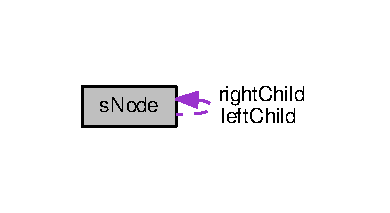
\includegraphics[width=187pt]{structsNode__coll__graph}
\end{center}
\end{figure}
\subsection*{Data Fields}
\begin{DoxyCompactItemize}
\item 
\hypertarget{structsNode_abc2af095ceb67883012bdae97f4c4537}{char $\ast$ {\bfseries command}}\label{structsNode_abc2af095ceb67883012bdae97f4c4537}

\item 
bool \hyperlink{structsNode_ad3ce64c185ce2fb0da1625cc6bce9803}{success}
\item 
char $\ast$ \hyperlink{structsNode_af404972110c1a3225dd689b03a931b36}{result}
\item 
char $\ast$ \hyperlink{structsNode_a114d95f7bc7d2ba888a7b297703d73dd}{separator}
\item 
char $\ast$ \hyperlink{structsNode_acaa42ae913310f65b9d08a4cecb3d40f}{input\-Value}
\item 
struct \hyperlink{structsNode}{s\-Node} $\ast$ \hyperlink{structsNode_abf2b6d71454df07a766b315346375dbd}{left\-Child}
\item 
struct \hyperlink{structsNode}{s\-Node} $\ast$ \hyperlink{structsNode_ad922ff3aa8dfeea7ca810d6524799126}{right\-Child}
\end{DoxyCompactItemize}


\subsection{Detailed Description}
noeud de l'arbre 

Noeud de l'arbre 

\subsection{Field Documentation}
\hypertarget{structsNode_acaa42ae913310f65b9d08a4cecb3d40f}{\index{s\-Node@{s\-Node}!input\-Value@{input\-Value}}
\index{input\-Value@{input\-Value}!sNode@{s\-Node}}
\subsubsection[{input\-Value}]{\setlength{\rightskip}{0pt plus 5cm}char$\ast$ s\-Node\-::input\-Value}}\label{structsNode_acaa42ae913310f65b9d08a4cecb3d40f}
chaine de caractère contenant le séparateur \hypertarget{structsNode_abf2b6d71454df07a766b315346375dbd}{\index{s\-Node@{s\-Node}!left\-Child@{left\-Child}}
\index{left\-Child@{left\-Child}!sNode@{s\-Node}}
\subsubsection[{left\-Child}]{\setlength{\rightskip}{0pt plus 5cm}struct {\bf s\-Node}$\ast$ s\-Node\-::left\-Child}}\label{structsNode_abf2b6d71454df07a766b315346375dbd}
chaine de caractère contenant le la valeur d'entré de la commande \hypertarget{structsNode_af404972110c1a3225dd689b03a931b36}{\index{s\-Node@{s\-Node}!result@{result}}
\index{result@{result}!sNode@{s\-Node}}
\subsubsection[{result}]{\setlength{\rightskip}{0pt plus 5cm}char$\ast$ s\-Node\-::result}}\label{structsNode_af404972110c1a3225dd689b03a931b36}
boolean indiquant le succés ou l'echec de la sous commande \hypertarget{structsNode_ad922ff3aa8dfeea7ca810d6524799126}{\index{s\-Node@{s\-Node}!right\-Child@{right\-Child}}
\index{right\-Child@{right\-Child}!sNode@{s\-Node}}
\subsubsection[{right\-Child}]{\setlength{\rightskip}{0pt plus 5cm}struct {\bf s\-Node}$\ast$ s\-Node\-::right\-Child}}\label{structsNode_ad922ff3aa8dfeea7ca810d6524799126}
fils droit \hypertarget{structsNode_a114d95f7bc7d2ba888a7b297703d73dd}{\index{s\-Node@{s\-Node}!separator@{separator}}
\index{separator@{separator}!sNode@{s\-Node}}
\subsubsection[{separator}]{\setlength{\rightskip}{0pt plus 5cm}char$\ast$ s\-Node\-::separator}}\label{structsNode_a114d95f7bc7d2ba888a7b297703d73dd}
chaine de caractère contenant le résultat de la commande \hypertarget{structsNode_ad3ce64c185ce2fb0da1625cc6bce9803}{\index{s\-Node@{s\-Node}!success@{success}}
\index{success@{success}!sNode@{s\-Node}}
\subsubsection[{success}]{\setlength{\rightskip}{0pt plus 5cm}bool s\-Node\-::success}}\label{structsNode_ad3ce64c185ce2fb0da1625cc6bce9803}
chaine de caractère contenant la commande 

The documentation for this struct was generated from the following file\-:\begin{DoxyCompactItemize}
\item 
src/\hyperlink{tree_8h}{tree.\-h}\end{DoxyCompactItemize}

\chapter{File Documentation}
\hypertarget{superbash_8c}{\section{src/superbash.c File Reference}
\label{superbash_8c}\index{src/superbash.\-c@{src/superbash.\-c}}
}


Programme principal du projet.  


{\ttfamily \#include $<$stdio.\-h$>$}\\*
{\ttfamily \#include $<$stdlib.\-h$>$}\\*
{\ttfamily \#include $<$string.\-h$>$}\\*
{\ttfamily \#include $<$stdbool.\-h$>$}\\*
{\ttfamily \#include $<$unistd.\-h$>$}\\*
{\ttfamily \#include \char`\"{}tree.\-h\char`\"{}}\\*
{\ttfamily \#include \char`\"{}logger.\-h\char`\"{}}\\*
Include dependency graph for superbash.\-c\-:
\nopagebreak
\begin{figure}[H]
\begin{center}
\leavevmode
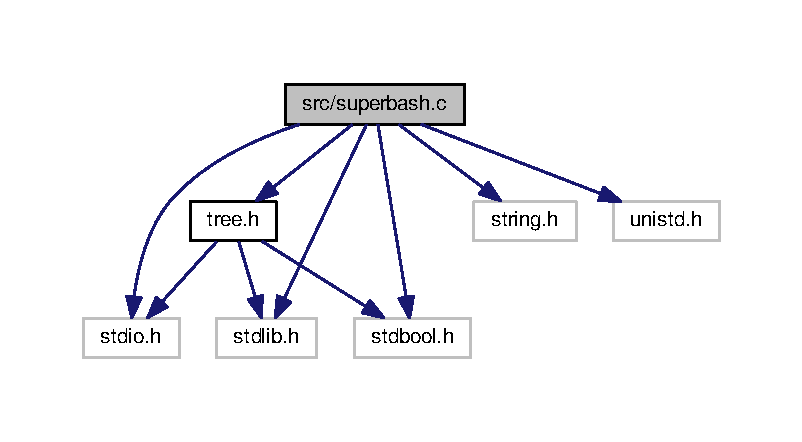
\includegraphics[width=350pt]{superbash_8c__incl}
\end{center}
\end{figure}
\subsection*{Macros}
\begin{DoxyCompactItemize}
\item 
\hypertarget{superbash_8c_acffba4e12894ca7015d00aaf3a2354cc}{\#define {\bfseries L\-S\-H\-\_\-\-R\-L\-\_\-\-B\-U\-F\-S\-I\-Z\-E}~1024}\label{superbash_8c_acffba4e12894ca7015d00aaf3a2354cc}

\end{DoxyCompactItemize}
\subsection*{Functions}
\begin{DoxyCompactItemize}
\item 
char $\ast$ \hyperlink{superbash_8c_a92c201a8e2d3381da8c1a9414d29e2d2}{substr} (char $\ast$src, int pos, int len)
\item 
char $\ast$ \hyperlink{superbash_8c_a0596c39f3cb05234e70ddae681b730a6}{read\-\_\-console\-\_\-line} (void)
\item 
void \hyperlink{superbash_8c_a40ea05e6559158264ffb3c0bcf215841}{bash\-\_\-loop} (void)
\item 
void \hyperlink{superbash_8c_a570d1340863a213574309e115443cf13}{trim\-Leading} (char $\ast$str)
\item 
void \hyperlink{superbash_8c_a8fa05a3f988073d4d9cc0de69a8b34ad}{trim\-Last} (char $\ast$str)
\item 
void \hyperlink{superbash_8c_a8ed89210277c9bc587916f95d08e023a}{remove\-\_\-space\-\_\-at\-\_\-beginning\-\_\-and\-\_\-end} (char $\ast$string)
\item 
\hyperlink{tree_8h_a37cd02a05176eff781378c1be7872b5b}{Node} $\ast$ \hyperlink{superbash_8c_a14cca885e3d4ae12aaf0c271cc82e5a2}{create\-\_\-tree\-\_\-from\-\_\-command} (char $\ast$command)
\item 
bool \hyperlink{superbash_8c_ac31b6205a5f05b1fd5fcb9646507b472}{read\-\_\-and\-\_\-exec\-\_\-tree} (\hyperlink{tree_8h_a37cd02a05176eff781378c1be7872b5b}{Node} $\ast$tree\-Command)
\item 
int \hyperlink{superbash_8c_af84467fe53452a65df671e6c1cee70f1}{handle\-\_\-command} (char $\ast$command)
\item 
int \hyperlink{superbash_8c_a370ffc4c27a249fb1029bdcdac48fec7}{execute\-\_\-command} (char $\ast$command)
\item 
void \hyperlink{superbash_8c_ab441892e9eec5b0ee1d6ece0f23594d3}{print\-\_\-current\-\_\-directory} ()
\item 
void \hyperlink{superbash_8c_a9b43697ad274f24cf39e6fe2ee7024da}{change\-\_\-current\-\_\-directory} (char $\ast$path)
\item 
\hypertarget{superbash_8c_a0ddf1224851353fc92bfbff6f499fa97}{int {\bfseries main} (int argc, char $\ast$argv\mbox{[}$\,$\mbox{]})}\label{superbash_8c_a0ddf1224851353fc92bfbff6f499fa97}

\end{DoxyCompactItemize}


\subsection{Detailed Description}
Programme principal du projet. \begin{DoxyAuthor}{Author}
Charly Mrazeck, Baptiste Oberbach 
\end{DoxyAuthor}
\begin{DoxyVersion}{Version}
0.\-1.\-0 
\end{DoxyVersion}
\begin{DoxyDate}{Date}
février 2018
\end{DoxyDate}
Programme executant le bash du projet superbash 

\subsection{Function Documentation}
\hypertarget{superbash_8c_a40ea05e6559158264ffb3c0bcf215841}{\index{superbash.\-c@{superbash.\-c}!bash\-\_\-loop@{bash\-\_\-loop}}
\index{bash\-\_\-loop@{bash\-\_\-loop}!superbash.c@{superbash.\-c}}
\subsubsection[{bash\-\_\-loop}]{\setlength{\rightskip}{0pt plus 5cm}void bash\-\_\-loop (
\begin{DoxyParamCaption}
\item[{void}]{}
\end{DoxyParamCaption}
)}}\label{superbash_8c_a40ea05e6559158264ffb3c0bcf215841}
Execute les commandes passé par ligne de commande \hypertarget{superbash_8c_a9b43697ad274f24cf39e6fe2ee7024da}{\index{superbash.\-c@{superbash.\-c}!change\-\_\-current\-\_\-directory@{change\-\_\-current\-\_\-directory}}
\index{change\-\_\-current\-\_\-directory@{change\-\_\-current\-\_\-directory}!superbash.c@{superbash.\-c}}
\subsubsection[{change\-\_\-current\-\_\-directory}]{\setlength{\rightskip}{0pt plus 5cm}void change\-\_\-current\-\_\-directory (
\begin{DoxyParamCaption}
\item[{char $\ast$}]{path}
\end{DoxyParamCaption}
)}}\label{superbash_8c_a9b43697ad274f24cf39e6fe2ee7024da}
Change le répertoire courant \hypertarget{superbash_8c_a14cca885e3d4ae12aaf0c271cc82e5a2}{\index{superbash.\-c@{superbash.\-c}!create\-\_\-tree\-\_\-from\-\_\-command@{create\-\_\-tree\-\_\-from\-\_\-command}}
\index{create\-\_\-tree\-\_\-from\-\_\-command@{create\-\_\-tree\-\_\-from\-\_\-command}!superbash.c@{superbash.\-c}}
\subsubsection[{create\-\_\-tree\-\_\-from\-\_\-command}]{\setlength{\rightskip}{0pt plus 5cm}{\bf Node}$\ast$ create\-\_\-tree\-\_\-from\-\_\-command (
\begin{DoxyParamCaption}
\item[{char $\ast$}]{command}
\end{DoxyParamCaption}
)}}\label{superbash_8c_a14cca885e3d4ae12aaf0c271cc82e5a2}
Créer un arbre à partir de la commande passé en paramètre \hypertarget{superbash_8c_a370ffc4c27a249fb1029bdcdac48fec7}{\index{superbash.\-c@{superbash.\-c}!execute\-\_\-command@{execute\-\_\-command}}
\index{execute\-\_\-command@{execute\-\_\-command}!superbash.c@{superbash.\-c}}
\subsubsection[{execute\-\_\-command}]{\setlength{\rightskip}{0pt plus 5cm}int execute\-\_\-command (
\begin{DoxyParamCaption}
\item[{char $\ast$}]{command}
\end{DoxyParamCaption}
)}}\label{superbash_8c_a370ffc4c27a249fb1029bdcdac48fec7}
Execute une commande \hypertarget{superbash_8c_af84467fe53452a65df671e6c1cee70f1}{\index{superbash.\-c@{superbash.\-c}!handle\-\_\-command@{handle\-\_\-command}}
\index{handle\-\_\-command@{handle\-\_\-command}!superbash.c@{superbash.\-c}}
\subsubsection[{handle\-\_\-command}]{\setlength{\rightskip}{0pt plus 5cm}int handle\-\_\-command (
\begin{DoxyParamCaption}
\item[{char $\ast$}]{command}
\end{DoxyParamCaption}
)}}\label{superbash_8c_af84467fe53452a65df671e6c1cee70f1}
Analyse la commande passé en paramètre et l'execute \hypertarget{superbash_8c_ab441892e9eec5b0ee1d6ece0f23594d3}{\index{superbash.\-c@{superbash.\-c}!print\-\_\-current\-\_\-directory@{print\-\_\-current\-\_\-directory}}
\index{print\-\_\-current\-\_\-directory@{print\-\_\-current\-\_\-directory}!superbash.c@{superbash.\-c}}
\subsubsection[{print\-\_\-current\-\_\-directory}]{\setlength{\rightskip}{0pt plus 5cm}void print\-\_\-current\-\_\-directory (
\begin{DoxyParamCaption}
{}
\end{DoxyParamCaption}
)}}\label{superbash_8c_ab441892e9eec5b0ee1d6ece0f23594d3}
Affiche le répertoire courant \hypertarget{superbash_8c_ac31b6205a5f05b1fd5fcb9646507b472}{\index{superbash.\-c@{superbash.\-c}!read\-\_\-and\-\_\-exec\-\_\-tree@{read\-\_\-and\-\_\-exec\-\_\-tree}}
\index{read\-\_\-and\-\_\-exec\-\_\-tree@{read\-\_\-and\-\_\-exec\-\_\-tree}!superbash.c@{superbash.\-c}}
\subsubsection[{read\-\_\-and\-\_\-exec\-\_\-tree}]{\setlength{\rightskip}{0pt plus 5cm}bool read\-\_\-and\-\_\-exec\-\_\-tree (
\begin{DoxyParamCaption}
\item[{{\bf Node} $\ast$}]{tree\-Command}
\end{DoxyParamCaption}
)}}\label{superbash_8c_ac31b6205a5f05b1fd5fcb9646507b472}
Lis un arbre et execute les commandes \hypertarget{superbash_8c_a0596c39f3cb05234e70ddae681b730a6}{\index{superbash.\-c@{superbash.\-c}!read\-\_\-console\-\_\-line@{read\-\_\-console\-\_\-line}}
\index{read\-\_\-console\-\_\-line@{read\-\_\-console\-\_\-line}!superbash.c@{superbash.\-c}}
\subsubsection[{read\-\_\-console\-\_\-line}]{\setlength{\rightskip}{0pt plus 5cm}char$\ast$ read\-\_\-console\-\_\-line (
\begin{DoxyParamCaption}
\item[{void}]{}
\end{DoxyParamCaption}
)}}\label{superbash_8c_a0596c39f3cb05234e70ddae681b730a6}
Lis une ligne de la console et renvois la ligne lu \hypertarget{superbash_8c_a8ed89210277c9bc587916f95d08e023a}{\index{superbash.\-c@{superbash.\-c}!remove\-\_\-space\-\_\-at\-\_\-beginning\-\_\-and\-\_\-end@{remove\-\_\-space\-\_\-at\-\_\-beginning\-\_\-and\-\_\-end}}
\index{remove\-\_\-space\-\_\-at\-\_\-beginning\-\_\-and\-\_\-end@{remove\-\_\-space\-\_\-at\-\_\-beginning\-\_\-and\-\_\-end}!superbash.c@{superbash.\-c}}
\subsubsection[{remove\-\_\-space\-\_\-at\-\_\-beginning\-\_\-and\-\_\-end}]{\setlength{\rightskip}{0pt plus 5cm}void remove\-\_\-space\-\_\-at\-\_\-beginning\-\_\-and\-\_\-end (
\begin{DoxyParamCaption}
\item[{char $\ast$}]{string}
\end{DoxyParamCaption}
)}}\label{superbash_8c_a8ed89210277c9bc587916f95d08e023a}
Enlève les espaces en début et en fin de chaine \hypertarget{superbash_8c_a92c201a8e2d3381da8c1a9414d29e2d2}{\index{superbash.\-c@{superbash.\-c}!substr@{substr}}
\index{substr@{substr}!superbash.c@{superbash.\-c}}
\subsubsection[{substr}]{\setlength{\rightskip}{0pt plus 5cm}char$\ast$ substr (
\begin{DoxyParamCaption}
\item[{char $\ast$}]{src, }
\item[{int}]{pos, }
\item[{int}]{len}
\end{DoxyParamCaption}
)}}\label{superbash_8c_a92c201a8e2d3381da8c1a9414d29e2d2}
retourne un string à partir de la string src à la position pos pour une longueur len \hypertarget{superbash_8c_a8fa05a3f988073d4d9cc0de69a8b34ad}{\index{superbash.\-c@{superbash.\-c}!trim\-Last@{trim\-Last}}
\index{trim\-Last@{trim\-Last}!superbash.c@{superbash.\-c}}
\subsubsection[{trim\-Last}]{\setlength{\rightskip}{0pt plus 5cm}void trim\-Last (
\begin{DoxyParamCaption}
\item[{char $\ast$}]{str}
\end{DoxyParamCaption}
)}}\label{superbash_8c_a8fa05a3f988073d4d9cc0de69a8b34ad}
Enlève les espaces en fin de chaine \hypertarget{superbash_8c_a570d1340863a213574309e115443cf13}{\index{superbash.\-c@{superbash.\-c}!trim\-Leading@{trim\-Leading}}
\index{trim\-Leading@{trim\-Leading}!superbash.c@{superbash.\-c}}
\subsubsection[{trim\-Leading}]{\setlength{\rightskip}{0pt plus 5cm}void trim\-Leading (
\begin{DoxyParamCaption}
\item[{char $\ast$}]{str}
\end{DoxyParamCaption}
)}}\label{superbash_8c_a570d1340863a213574309e115443cf13}
Enlève les espaces en début de chaine 
%--- End generated contents ---

% Index
\newpage
\phantomsection
\addcontentsline{toc}{chapter}{Index}
\printindex

\end{document}
